\documentclass[12pt,letterpaper]{article}
\input macawlrs.tex
\newcommand{\jd}[1]{\textcolor{blue}{${\textrm{Julio: }}${#1}}}

\usepackage[scale=0.845]{geometry}


%\usepackage[urw-garamond]{mathdesign}
%\usepackage[T1]{fontenc}

\usepackage[cmintegrals,cmbraces]{newtxmath}
\usepackage{ebgaramond-maths}
\usepackage[T1]{fontenc}
\usepackage{svg}


\usepackage{fancyheadings}
\usepackage{lastpage}
\lhead{\tt Deride-Ram\'irez - Working note}
\chead{\tt SNL-FRB}
\rhead{\tt \today}
\cfoot{\tt \small Page \thepage\ of \pageref{LastPage}}

\pagestyle{fancyplain}


\usepackage{lineno}
\linenumbers

\title{A Model for Robust Regulation of Financial Networks}
\usepackage{authblk}
\author[1]{Julio Deride \thanks{jaderid@sandia.gov}}
\author[2]{Carlos Ram\'irez \thanks{carlos.ramirez@frb.gov}}
\affil[1]{Sandia National Laboratories, USA}
\affil[2]{Federal Reserve Board, USA}
\renewcommand\Authands{ and }

\begin{document}
\maketitle
\baselineskip=15pt

\begin{abstract}
We develop a model to study the problem of a social planner who seeks to regulate a financial network in which shocks propagate across firms while she is unsure about the underlying network structure. We derive her optimal policy as a function of investors' attitudes towards risk and ambiguity, firms' information sets, and invariant network characteristics. Our preliminary results highlight the importance of uncertainty and firms' information sets on the optimal policy intervention.
\end{abstract}

\section{Problem}
Consider a network $\rsG=(V,\,E)$ consisting on a set of $n$ nodes, $V=\{1,\ldots,n\}$, and a set of $m$ undirected edges $\{e_{ij}\}\in E$. Each node $i$ represents one of the institutions identity, and each edge $e_{ij}$ represents the \emph{correlation} or contagion factor between two entities. Let $(\Omega,\rsA,\Pro)$ be a probability space ...


Consider a two-stage model, where on the first stage there is a random shock happening on the nodes.   Let $\xi_i$ a Bernoulli random variable such that $\xi^0_i\in\{0,1\},\,i=1,\ldots,n$ represents the \emph{distress state} of node-$i$ on the network.  On the other hand, the second stage captures the behavior of the \emph{shock's propagation} over the network.  In order to define this, consider the stochastic process ${\bf P}$ modeling the probability of contagion of a node, given that one of its neighbor is distressed, i.e., if $\xi^1_i\in\{0,\,1\}$ represents the distress state of node $i$ in the second stage, then
\[{\bf P}_{ij}=\Pro\lset \xi^1_i(\cdot)=1\,\mset\,\xi^0_j=1\rset\,\quad e_{ij}\in E,\,\forall i,j\in V\]

The problem is now to minimize the total cost of the system under shocks on the network.  For this, the regulator is set to solve the problem of minimizing an overall cost, consisting on implementation cost and contagion cost, by deciding an optimal capital requirement.  Let $x^0$ be the decision policy, $x^0\in[0,1]^n$ such that $x^0_i$ represents the policy required at entity $i$, and ${\bf x}^1(\cdot)$ be a decision policy regarding the second stage (not sure if needed or not).  The optimization problem is given by
\[(\rsP)\quad \begin{array}{rl}\min_{\{x^0,{\bf x}^1(\cdot)\}}&\phi^0(x^0)+\Ex\lset \phi^1(\cdot,x^0,{\bf x}^1(\cdot))\rset\\
\suchthat&f^0(x^1)\leq 0 \\
&f^1(x^0,{\bf x}^1(\omega),\omega)\leq 0,\,\omega-\as\\
&x^0\in[0,1]^n,\,x^1:\Omega\to\reals^N\end{array},\]
where $\phi^0$ is the total cost of implementing a capital requirement policy, and $\phi^1$ is the total cost of the second stage (probably related to the contagion cost). Here, the network constraints are included in the constraints $\{f^0,f^1\}$ and for a random realization $\omega$ and a given policy $x^1$, the cost $\phi(\omega,x^0,{\bf x}^1(\omega))$ should reflect the cost of the contagion on the system. For example, one can be interested in minimizing the expected cost of the contagion, but it is easy to incorporate a risk-measure for minimizing, for example, a measure like $C-Var$ of the tail of the distribution of distressed nodes.

\section{Tue, Feb 20th}
We explore a model with the following features
\begin{itemize}
\item[1.] Consider a graph $G=(N,E)$, where each node represents a financial institution, and each edge reflects financial transactions between two institutions. 

\item[2.] Instituion $i$ faces a financial shock, represented as $\epsilon_i$, which impacts its assets over liabilities ratio, defined as $r_i=\frac{A_i}{L_i}$, \footnote{Capital?}.  Additionally, we consider that a financial institution is under \emph{distress} if its ratio is under a (given) threshold $\lambda\in(0,1)$.  Thus,
\[i\;{\rm under\,distress}\iff r_i(1-\epsilon_i)<\lambda\]

\item[3.] There is a central decision maker, focus on the stability of the system.  We discussed the information that is available to this regulator, and propose a mechanism to oversee the overall stability within the financial network thorugh a constraint over the ratio, given by $x_i$.

\item[4.]  The financial institutions decide their ratio by maximizing their profits\footnote{utility?}, given by a function $\pi_i$, with the minimum level of A/L ratio, i.e.,
\[r_i(x_i;p)\in\argmax_r\lset \Ex^p\{ \pi(r)\}\mset r\geq x_i,\,r\in R_i\rset\]
Additionally, assuming that the function $\pi_i$ is nonincreasing on $r$ (and no further restrictions are imposed), the individual solution to this problem is given by $r_i^*=x_i$, i.e., the financial institution sets its ratio at minimum possible level.

\item[5.] There is contagion on the network, described in its stationary state as follows: if institution $i$ gets distressed, there is a probability $p$ that it affects its immediate neighbor, $p^2$ by a 2-edge neighbors, and so on.  Defining the set $\{j\to i\}$ as the set of all possible simple paths coming to node $i$, and $d(j,i)$ the distance between $j$ and $i$ (amount of edges between them), the expected shock\jd{Assuming that there is no \emph{amplification} of shocks} is given by
\[\epsilon_i=\sum_{j\to i} p^{d(i,j)}\epsilon_j\]
and by defining the matrix $A_{ij}=\sum_{j\to i} p^{d(i,j)}$, the acceptable shocks are the solution of the eigen problem for the matrix $A$.  Moreover, we interpret $A$ as an stochastic (transition) matrix by enlarging it with an extra \emph{not distressed} node as follows,
\[\Tilde A=\left[\begin{array}{c|cccc|c}
&1&2&\ldots&n&ND\\
\hline
1&0&\sum_{2\to 1} p^{d(2,1)}&\ldots&\sum_{n\to 1} p^{d(n,1)}&1-\sum A_{1\cdot}\\
\vdots&\vdots&\ddots&\vdots&\vdots\\
n&\sum_{n\to 1} p^{d(n,1)}&\vdots&\ldots&0&1-\sum A_{1\cdot}\\
\hline
ND&0&0&0&0&1
\end{array}\right]\] 
This is a stochastic matrix, and thus, it has an eigenvalue with value 1, wich associated eigenvector $\tilde \epsilon^0$.  Let's consider the first $n$ components as acceptable shocks $\epsilon^0$ for the corresponding nodes.
\item Finally, consider the optimization problem solved by the central planner: set the ratio level\jd{sth about the condition previously stated}, such that it minimizes the total amount of financial institutions under distress.  Let $y_i\in\{0,1\}$ a binary variable such that $y_i=1$ if insititution $i$ is under distress or $y_i=0$ otherwise, and let $M>0$ large enough such that
\begin{align}\label{form1}
\min_{x,y}&\,\sum_{i=1}^n y_i+\phi(x,y)\\
\suchthat&r_i(x_i)(1-\epsilon^0_i)-\lambda\leq M(1-y_i),\,i=1,\ldots,N
\end{align}
where $\phi$ is a cost function associated to the policy $x$ and the instituions on distress.  Note that this formulation depends on $p$ and the topology of the network through the selection of the $\epsilon^0$.
\item The optimization problem \ref{form1} can have a robust formulation by considering an ambiguity set for the parameter $p$, thus
\begin{align}\label{formr1}
\min_{x,y}\sup_{p\in\cA(p_0)}&\,\sum_{i=1}^n y_i+\phi(x,y)\\
\suchthat&r_i(x_i)(1-\epsilon^0_i)-\lambda\leq M(1-y_i),\,i=1,\ldots,N
\end{align}
\item Finally, we are looking for a representative agent formulation of the benevolent social planner problem, such that the solutions of both problems coincide.  For example, one wild guess is to consider the formulation proposed in \cite{?} \jd{Citation needed}, where ambiguity is considered as a  family of possible models for the parameter $p$, along with a probability distribution over these models, $\alpha$.  Therefore, the central planner problem has the following form
\[\max_x\Lset \Ex^p\Lset\sum_i u_i(x_i)\Rset -\frac{\mu}{2}{\rm Var}^p\left(\sum_i u_i(x_i)\right)-\frac{\theta}{2}{\rm Var}_\alpha\Ex\left(\sum_i u_i(x_i)\right)\Rset\] 
\end{itemize}
\section{Wed, Feb 21st}
Continuing the idea of a (benevolent) central planner, let's define the following modified utility functions for each agents:
\[\tilde{\pi}_i=\begin{cases} \pi_i&{\rm institution}\,i\,{\rm operates\,normally}\\
0&{\rm institution\,is\,on\,distress}\end{cases}\]
Therefore, we expect that the Central Planner solves the following problem
\[\max_x\Lset \Ex^p\Lset\sum_i \tilde\pi_i(x_i)\Rset -\frac{\mu}{2}{\rm Var}^p\left(\sum_i \tilde\pi_i(x_i)\right)-\frac{\theta}{2}{\rm Var}_\alpha\Ex\left(\sum_i \tilde\pi_i(x_i)\right)\Rset\]

Additionally, we modify the assumptions over the spread of the distress condition

\begin{assumption}{\rm (initial shocks)}\label{assinit}
Initial shock only affects one institution (node)
\end{assumption} 

\begin{assumption}{\rm (propagation)}\label{assprop}
Propagation occurs over simple paths
\end{assumption} 

Under Assumptions~(\ref{assinit},\ref{assprop}), one can formulates the probaility of distress of node $k$, $\Pro\{D_k\}$, by a simple recursion.  If $j$ and $i$ are directly connected, the probability is given by
\begin{eqnarray*}
\Pro_{j|i}&=&\Pro\{D_j|D_i\}\\
&=&\Pro\{r_j(1-\epsilon_j)<\lambda|D_i\}\\
&=&\Pro\{r_j(1-p\epsilon_i)<\lambda|D_i\}\\
&=&1-F_{\epsilon_i}\left(\frac{1}{p}\left(1-\frac{\lambda}{r_j}\right)\right)
\end{eqnarray*}
where $F_{\epsilon_i}$ corresponds to the cdf of $\epsilon_i$.  Finally, for every institution (node) of the network, the contagion will depend only on all the possible simple paths connecting the corresponding node and the initially infested \jd{?}. Therefore,
\begin{equation}
\Pro\{D_k\}=\sum_{l\to k} \Pro\{D_k|D_l\}\cdot\Pro\{D_l\}
\end{equation}

\subsection{Revisiting the institutions' problem}
Let's consider an stochastic problem, where each node $i$ faces uncertainty on the final ratio.  Denote as $\epsilon$ the random shock that the agent expects ($\Ex \epsilon=\bar\epsilon>0$), and assume that every agent is risk neutral \jd{focused on network effects} and their profits are homogeneous and linear: $\pi(r)=a^0-a^1\,r$, $a^0,a^1>0$. Thus, the agent maximization problem is given by
\[r_i(x_i;\bar \epsilon)\in\argmax_r\lset \Ex\{ \pi(r(1-\epsilon))\}\mset r\geq x_i,\,r\in R_i\rset\]

Additionally, we include explicitly the participation constraint, where agent-$i$ only participates in the economy if its expected profits are nonnegative.  
\[r_i(x_i;\bar \epsilon)\in\argmax_r\lset a^0-a^1(1-\bar\epsilon)r\mset r\geq x_i,\,r\in R_i,\,a^0-a^1(1-\bar\epsilon)r\geq 0\rset\]

Note that in this formulation we consider agents that proceed in a \emph{na\"ive} fashion by only maximizing their profits, without considering its exposure within the network.

Following steps: Solve the problem considering
\begin{enumerate}
\item Risk neutral CP
\item Risk averse and Ambiguity neutral
\item Risk averse and Ambiguity averse
\item Numerical example
\end{enumerate}


\section{Toy Model}

\subsection{Parameters}
\begin{itemize}
\item[$a^0$]
\item[$a^1$]
\item[$\lambda$]
\item[$F_\epsilon$]
\end{itemize}

\section{Thu, Feb 22}
We realize that the only important condition for distress is given by the interaction of each node with its immediate neighbors.  Consider the institution $n$, and denote by $\cN(n)$ the set of its neighbors, i.e., nodes that directly connect to $n$, and let $q_n$ be the probability that institution $n$ faces an idiosyncratic shock.  Therefore, the probability of $n$ entering the distress condition, $D_n$,  is given by
\[\Pro\{D_n\} = q_n p^0_n+\sum_{m\in \cN(n)} \Pro\{D_n|D_m\}\Pro\{D_m\},\]
where the first component of the sum reflects the distress due to a idiosyncratic shock to the institution $n$, and the associated probability of entering distress,  $p^0_n=\Pro\{r_n(1-\epsilon)<\lambda\}$, and the second component is the {\bf network effect}, i.e., the probability of the contagion through the connection to the network.

Using matrix notation, define the matrix $\Gamma_{ij}=\Pro\{D_i|D_j\}$ for each $(i,j)\in E$, and zero otherwise. Then, the probabilities of distress are the solution of the system
\begin{equation}\label{transprob}
P=qp^0+\Gamma\,P\quad \Rightarrow \quad P=(I-\Gamma)^{-1}(qp^0)
\end{equation}

Additionally, this equation imposes implictly conditions over the parameters of the problems such that the solution is a vector of probabilities.  We need to focus our attention to set of parameters such that the matrix $\Gamma$ satisfies the following condition 
\[(I-\Gamma)^{-1}(qp^0) \in [0,1]^N\]

\section{Optimal value of profits}
For the CP problem, the expected utility is given by
\[\Ex\{\tilde\pi^*_i(x_i)=\Ex \Ex\{ \tilde\pi^*_i(x_i)|~D_i\}\]
\section{Fri, Feb 23rd}
\[r_i(x_i;F_\epsilon(p,\cN))\in\argmax_r\lset \Ex\{ \pi(r(1-\epsilon))\}\mset r\geq x_i,\,\Ex\{ \pi(r(1-\epsilon))\}\geq 0\rset\]
\subsection{Analyzing the shock}
The shock have two possible sources: Idiosyncratic $\epsilon^I$, and Non-Idiosyncratic (coming from the network), $\epsilon^{Nt}$.  For insititution $i$, the probability of receiving the idiosyncratic shock is given by $q_i$, and we assume that $\epsilon_i^I\sim {\rm U}[0,UB]$, and that 
\[\epsilon=\begin{cases}
\epsilon^I&\Pro\{\cdot\}=q_i\\
\epsilon^{Nt}&1-q_i
\end{cases}\]

We realize that the contagion mechanism and the shock propagation are going to be analyzed with different perspective
\begin{itemize}
\item The idiosyncratic risk can be initiated at node $i$ with probability $q_i$
\item Once the institution $i$ receives the shock, it propagates it with an intensity of $p$ times the shock \jd{note that here, we can consider $p<1$ for mitigation effect, or $p>1$ for an increasing effect}. 
\item The shock only propagates by simple paths between nodes (no revisiting allowed)

\begin{assumption}{\rm (shock propagation)}\label{assshprop}
The shock {\bf always propagates}, independently of the distress condition of the institution.
\end{assumption}
\item The final form for the shock faced by each institution is given by the equation
\begin{equation}\label{eqshockprop}
\epsilon = \left(\sum_{n=1}^{|N|-1} p^nA^n+I\right)q\epsilon^I
\end{equation}
\end{itemize}

\jd{Check the information available for each agent: Is the node totally visible for each agent?} We will continue assuming perfect information wrt the network

\subsection{$i$-maximization problem}
Define the {\emph modified agent maximization problem}
\begin{align*}
\max_r&\;\Ex\{ \pi(r(1-\epsilon))\}\\
\suchthat&\;r\geq x,\\
&\;\Ex\{ \pi(r(1-\epsilon))\}\geq 0,
\end{align*}
where $\epsilon$ comes from Equation~(\ref{eqshockprop}).  Note that by the linearity of the propagation, $\epsilon$\footnote{Simple paths?} followed the distribution of $\epsilon^I$, modified by a constant (easy to compute).  Thus, define these coefficients as $S_i$\footnote{$S=(\sum p^nA^n+I)q$}, and let's compute the expectation, 
\[\pi(\tau)=\begin{cases}a^0-a^1\tau& \tau\geq \lambda\\ 0&{\rm o.w.}\end{cases}\]
\begin{eqnarray*}
\Ex\{ \pi(r(1-\epsilon))\}&=&\Ex\lset\,\Ex\{ \pi(r(1-\epsilon))|r(1-\epsilon)\geq\lambda\}+\Ex\{ \pi(r(1-\epsilon))|r(1-\epsilon)<\lambda\}\rset\\
&=&\left(\int_{\{\epsilon:r(1-\epsilon)\geq \lambda\}}(a^0-a^1r(1-\tau))\Pro(d\tau) \right)\Pro\{r(1-\epsilon)\geq\lambda\}\\
&=&\begin{cases}
0&1-\frac{\lambda}{r}\leq 0\\
a^0-a^1r(1-\Ex\{\epsilon\})&\frac{1}{S\cdot UB}\left(1-\frac{\lambda}{r}\right)\geq 1\\
\left(1-\frac{\lambda}{r}\right)\int_0^{1-\frac{\lambda}{r}}(a^0-a^1r(1-t))\,\frac{dt}{S\cdot UB}&{\rm o.w.}
\end{cases}\\
&=&\begin{cases}
0&1-\frac{\lambda}{r}\leq 0\\
a^0-a^1r(1-\Ex\{\epsilon\})&\frac{1}{S\cdot UB}\left(1-\frac{\lambda}{r}\right)\geq 1\\
\frac{1}{S^2\cdot UB^2}\left(1-\frac{\lambda}{r}\right)^2(a^0-a^1\frac{r+\lambda}{2})\,&{\rm o.w.}
\end{cases}
\end{eqnarray*}
\section{Wed, Feb 28th}
The computation of the expectation is
\begin{eqnarray*}
\Ex\{ \pi(r(1-\epsilon))\}&=&\begin{cases}
0&1-\frac{\lambda}{r}\leq 0\\
a^0-a^1r(1-\Ex\{\epsilon\})&\frac{1}{S\cdot UB}\left(1-\frac{\lambda}{r}\right)\geq 1\\
\frac{1}{(S\cdot UB)^2}\left(1-\frac{\lambda}{r}\right)^2(a^0-a^1r\left(1-\frac{1}{2}\left(1-\frac{\lambda}{r}\right)\right)\,&{\rm o.w.}
\end{cases}
\end{eqnarray*}
Note that this function is continuous.  The optimal value for $x\geq 0$ is given by
\begin{equation}
r^*(x)\in\argmax_r \lset \Ex\{ \pi(r(1-\epsilon))\}\mset r\geq x, \Ex\{ \pi(r(1-\epsilon))\}\geq 0\rset = \begin{cases}
\emptyset & x\geq \frac{a^0}{a^1}\frac{1}{1-\Ex\{\epsilon\}}\\
\frac{\lambda}{1-S\cdot UB}& 0\leq x<\frac{\lambda}{1-S\cdot UB}\\
x& \mbox{o.w}\end{cases}
\end{equation}
The function $\Ex\{ \pi(r(1-\epsilon))\}$ is depicted in Figure~(\ref{figExUt}).  From here it is easy to see that the optimum of the optimization problem depends on the values of $x$.

\begin{figure}[htbp] %  figure placement: here, top, bottom, or page
   \centering
   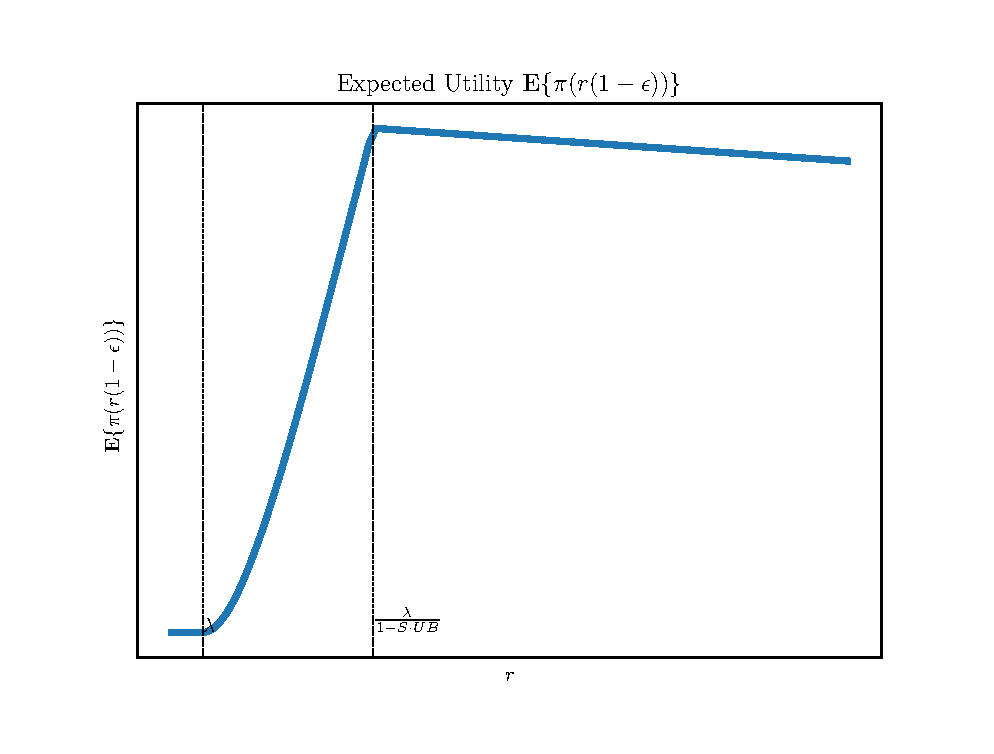
\includegraphics[width=0.7\textwidth]{ExpectedUt} 
   \caption{Expected utility}
   \label{figExUt}
\end{figure}

Finally, the optimal expected utility is given by
\begin{equation}\label{eqEPOpt}
\Ex\pi\{r^*(x)(1-\epsilon)\}=\begin{cases}
a^0-a^1x(1-\Ex\{\epsilon\})&\frac{\lambda}{1-S\cdot UB}\leq x\leq \frac{a^0}{a^1}\frac{1}{1-\Ex\{\epsilon\}}\\
a^0-a^1\frac{\lambda}{1-S\cdot UB}(1-\Ex\{\epsilon\})&0\leq x\leq \frac{\lambda}{1-S\cdot UB}\\
0&{\rm ow}
\end{cases}
\end{equation}
and it's depicted on Figure~(\ref{figOpExUt}).

\begin{figure}[htbp] %  figure placement: here, top, bottom, or page
   \centering
   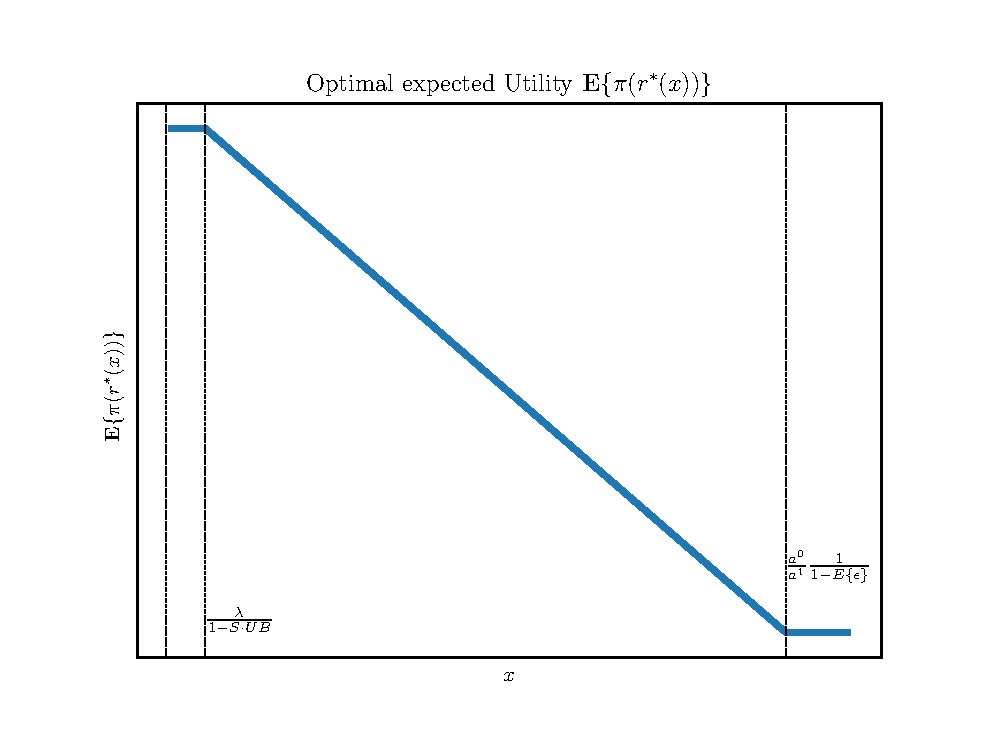
\includegraphics[width=0.7\textwidth]{OptExpUt} 
   \caption{Optimal Expected utility}
   \label{figOpExUt}
\end{figure}

\section{Thu, Mar 1st}
\subsection{CP Problem}
Assuming a risk-averse central planner, we can compute the individual variance by
considering different cases
\begin{description}
\item[$x_i\in(0,\lambda_i=\frac{\lambda}{1-S_i\cdot UB})$]
In this case, the optimal rule corresponds to $r_i^*(x_i)=\lambda_i$ and the final expression of the variance does not depend on $x$. Nevertheless, it is given by
\[\var\{\pi_i(r^*_i(x_i)(1-\epsilon_i))\}=\displaystyle\begin{cases}
(a_1\lambda_i)^2\frac{(S_i\cdot UB)^2}{12}&1-\frac{\lambda}{\lambda_i}>S_i\cdot UB\\
0&1-\frac{\lambda}{\lambda_i}<0\\
\left(1-\frac{\lambda}{\lambda_i}\right)(a_1\lambda_i)^2\int_0^{1-\frac{\lambda}{\lambda_i}}(\tau-\Ex\epsilon)^2\Pro(d\tau)&{\rm o.w.}
\end{cases}\]

\item[$x_i\in(\lambda_i,\frac{a^0}{a^1}\frac{1}{1-\Ex\epsilon})$] Here, $r_i^*(x_i)=x_i$
\begin{eqnarray*}
\var\{\pi_i(r^*_i(x_i)(1-\epsilon_i))\}&=&\begin{cases}
(a_1 x)^2\frac{(S_i\cdot UB)^2}{12}&x\geq \lambda_i\\
\left(1-\frac{\lambda}{x}\right)^2\frac{(a_1\,x)^2}{3\,S_i\cdot UB}\left(\left(1-\frac{\lambda}{x}-\frac{S_i\cdot UB}{2}\right)^2-\frac{S_i\cdot UB}{2}\left(1-\frac{\lambda}{x}-\frac{S_i\cdot UB}{2}\right)+\left(\frac{S_i\cdot UB}{2}\right)^2\right)&{\rm o.w.}
\end{cases}
\end{eqnarray*}
\end{description}
\jd{check the regions!}

\subsection{Individual Variances}
The individual variance is given by
\begin{equation}\label{indvar}
\var\{\pi_i(r^*_i(x_i)(1-\epsilon_i))\}=\begin{cases}
(a_1\lambda_i)^2\frac{(S_i\cdot UB)^2}{12}&\lambda\leq x\leq \lambda_i\\
(a_1 x)^2\frac{(S_i\cdot UB)^2}{12}&\lambda_i\leq x\leq 1\\
0& {\rm ow}
\end{cases}
\end{equation}

\subsection{Pairwise Covariances}
Consider the nodes $i$ and $j$.  The covariance of the profits between these two institutions can be decompsed according to the values of $x_i$ and $x_j$.  It's easier to see this on the Figure~(\ref{figcovzones}).

\begin{figure}[htbp]
   \centering
   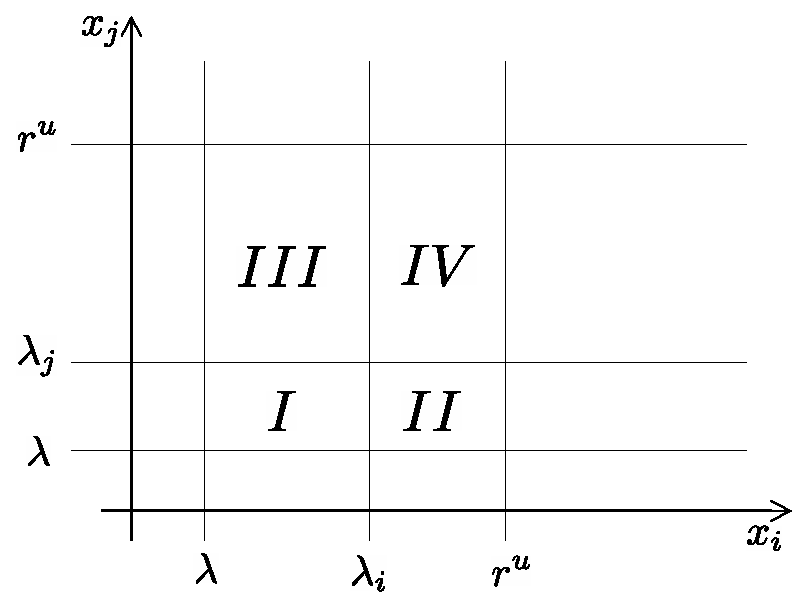
\includegraphics[width=0.5\textwidth]{CovAreas} % requires the graphicx package
   \caption{Areas for Covarianes}
   \label{figcovzones}
\end{figure}

After some algebra, the final form of the covariances is given by
\begin{equation}\label{eqcovij}
\cov(\pi_i(r^*_i(x_i(1-\epsilon_i))),\pi_j(r^*_j(x_j(1-\epsilon_j))))=\begin{cases}
(a_1)^2S_iS_j\lambda_i\lambda_j\frac{(UB)^2}{12}&\lambda\leq x_i\leq\lambda_i,\,\lambda\leq x_j\leq\lambda_j,(I)\\
(a_1)^2S_iS_j x_i\lambda_j\frac{(UB)^2}{12}&\lambda_i\leq x_i\leq r^u,\,\lambda\leq x_j\leq\lambda_j,(I)\\
(a_1)^2S_iS_j \lambda_i x_j\frac{(UB)^2}{12}&\lambda\leq x_i\leq \lambda,\,\lambda_j\leq x_j\leq r^u,(III)\\
(a_1)^2S_iS_j x_i x_j\frac{(UB)^2}{12}&\lambda_i\leq x_i \leq r^u \lambda,\,\lambda_j\leq x_j\leq r^u,(IV)\\
0&{\rm ow}
\end{cases}
\end{equation}

\jd{Note} By definition of the matrix $S$, it can be interpreted as the truncation of an exponential matrix
\[S=(\sum_{n=1}^{N-1} (pA)^n+I)q=(\sum_{n=0}^{N-1} (pA)^n)q \approx {\rm e}^{pA}q,\]
although if we rule out cycles, technically, the matrix does not have elements on the diagonal, thus, it is not $A$

\subsection{Risk-neutral Central Planner}
Recall the following definitions
\[S=\sum_{n=0}^{N-1}(pA)^nq,\quad \epsilon^I\sim{\rm U}(0,UB),\quad \lambda_i=\frac{\lambda}{1-S_i\cdot UB}, \quad r^u=\frac{a^0}{a^1}\frac{1}{1-\Ex\epsilon}\]
The risk-neutral CP maximizes the following function
\begin{equation}\label{rnutfun}
\begin{align}
f(x)&=\Ex\Lset \sum_{i=1}^N \pi_i(r^*_i(x_i)(1-\epsilon_i))\Rset\\
&=\sum_{i=1}^N \Ex\Lset\pi_i(r^*_i(x_i)(1-\epsilon_i))\Rset\\
&=\sum_{i=1}^N \begin{cases}
a^0-a^1\lambda_i(1-\Ex\{\epsilon\})&0\leq x_i\leq \lambda_i\\
a^0-a^1x_i(1-\Ex\{\epsilon\})&\lambda_i\leq x_i\leq r^u\\
0&{\rm ow}
\end{cases}
\end{align}
\end{equation}
Here, we have two cases: the CP is allowed to impose individual constraints $x_i$, or a general rule $x_i=x,\forall i$. The solution to these problems:
\begin{description}
\item[Individual policy] In this case, the problem of maximizing the function $f(x)$ defined in Equation~(\ref{rnutfun}) is separable, and the solution is given by
\begin{equation}\label{solrncpproind}
\max_{(x_1,\ldots,x_N} f(x)\iff x_i^*\in\argmax \Ex\pi_i(r^*_i(x_i)(1-\epsilon_i))=[0,\lambda_i],\,i=1,\ldots,N
\end{equation}

\item[Global policy] In this case, the CP is only able to choose one value of $x$ for every node of the network.  Therefore, the solution that maximizes the utility is given by
\begin{equation}\label{solrncpproglo}
\max_{x} f(x)\iff x^*\in\argmax \sum_i\Ex\pi_i(r^*_i(x)(1-\epsilon_i))=[0,\min_{i=1,\ldots,N}\{\lambda_i\}]
\end{equation}
\end{description}
\jd{Note that this analysis always incorporates that the agents internalize the non-default condition, i.e., if the policy $x$ is too low, they natural move their optimal level to the one that avoid the default case}
\section{Mon, Mar 5th}
\subsection{Toy example}
Consider the following economy, 
\[N=\{0,1,2\},\quad E=\{(0,1),(1,2)\},\quad \lambda=5\%,\quad UB=\frac{1}{4},\quad p=\frac{1}{2},\quad a_0=a_1=1,\quad q_0=q_1=q_2=\frac{1}{3},\]
this easy example is depicted in Figure~(\ref{figToyNtw})
\begin{figure}[htbp]
   \centering
   
\includegraphics[width=0.9\textwidth]{ToyNtw} % requires the graphicx package
   \caption{Toy example}
   \label{figToyNtw}
\end{figure}
For this economy, we we first compute
\begin{eqnarray*}
\Ex\epsilon&=&\frac{1}{8},\\
S_0=S_2&=&\frac{1}{n}\{1+p+p^2\}\\
&=&\frac{7}{12}\\
S_1&=&\frac{1}{n}\{p+1+p\}\\
&=&\frac{2}{3}\\
\lambda_0=\lambda_2&=&\frac{\lambda}{1-S_0\cdot UB}\\
&=&\frac{12}{205}\approx 5.85\%\\
\lambda_1&=&\frac{\lambda}{1-S_1\cdot UB}\\
&=&\frac{6}{100}=6\%\\
r^u&=&\frac{a_0}{a_1}\frac{1}{1-\Ex\epsilon}\\
&=&\frac{8}{7}
\end{eqnarray*}
and we have the following features:
\begin{description}
\item[Expected utility] Using Equation~(\ref{}), we have
\begin{eqnarray*}
\Ex\pi_0\{r_0^*(x)(1-\epsilon)\}=\Ex\pi_2\{r_2^*(x)(1-\epsilon)\}&=&\begin{cases}
\frac{389}{410}&0\leq x\leq \frac{12}{205}\\
1-\frac{7}{8}x&\frac{12}{205}\leq x\leq \frac{8}{7}\end{cases}\\
\Ex\pi_1\{r_1^*(x)(1-\epsilon)\}&=&\begin{cases}
\frac{379}{400}&0\leq x\leq \frac{6}{100}\\
1-\frac{7}{8}x&\frac{6}{100}\leq x\leq \frac{8}{7}\end{cases}\\
\end{eqnarray*}
\item[Variances] Using Equation~(\ref{}), we have
\begin{eqnarray*}
\var\pi_0\{r_0^*(x)(1-\epsilon)\}=\var\pi_2\{r_2^*(x)(1-\epsilon)\}&=&\begin{cases}
\frac{1}{12}\left(\frac{12}{205}\right)^2\frac{49}{48^2}&0\leq x\leq \frac{12}{205}\\
\frac{1}{12}x^2\frac{49}{48^2}&\frac{12}{205}\leq x\leq 1\end{cases}\\
\var\pi_1\{r_1^*(x)(1-\epsilon)\}&=&\begin{cases}
\frac{1}{12}\left(\frac{6}{100}\right)^2\frac{1}{36}&0\leq x\leq \frac{6}{100}\\
\frac{1}{12}x^2\frac{1}{36}&\frac{6}{100}\leq x\leq 1\end{cases}\\
\end{eqnarray*}
\item[Covariances] Using Equation~(\ref{}) we have
\begin{eqnarray*}
\cov(\pi_0(x_0),\,\pi_2(x_2))&=&\begin{cases}
\left(\frac{7}{12}\right)^2 \left(\frac{12}{205}\right)^2 \frac{1}{12\cdot 16}&0\leq x_0 \leq \frac{12}{205},\,0\leq x_1\leq \frac{12}{205}\\
\left(\frac{7}{12}\right)^2 \frac{12}{205} \frac{1}{12\cdot 16}x_0&\frac{12}{205}\leq x_0 \leq 1 ,\,0\leq x_1\leq \frac{12}{205}\\
\left(\frac{7}{12}\right)^2 \frac{12}{205} \frac{1}{12\cdot 16}x_2&0\leq x_0 \leq 1 ,\,\frac{12}{205}\leq x_1\leq \\
\left(\frac{7}{12}\right)^2  \frac{1}{12\cdot 16}x_0x_2&\frac{12}{205}\leq x_0 \leq 1,\,\frac{12}{205}\leq x_1\leq 1
\end{cases}\\
\cov(\pi_0(x_0),\pi_1(x_1))&=&\begin{cases}
\frac{7}{3\cdot 205\cdot 100\cdot 16}&0\leq x_0 \leq \frac{12}{205},\,0\leq x_1\leq \frac{6}{100}\\
\frac{7}{3\cdot 100\cdot 12\cdot 16}x_0&\frac{12}{205}\leq x_0 \leq 1 ,\,0\leq x_1\leq \frac{6}{100}\\
\frac{7}{6\cdot 3\cdot 205\cdot 16}x_1&0\leq x_0 \leq 1 ,\,\frac{6}{100}\leq x_1\leq \\
\frac{7}{6\cdot 3\cdot 12\cdot 16}x_0x_1&\frac{12}{205}\leq x_0 \leq 1,\,\frac{6}{100}\leq x_1\leq 1
\end{cases}
\end{eqnarray*}
\end{description}


\section{Thu, Mar 8th}
\subsection{Computing the ambiguity term}
In this subsection we're interested in computing the term corresponding to the ambiguity of the CP.  Recall that we introduce ambiguity on the rate of the shock contagion, ${\bf p}$, where now we consider that it can have different values, $p_0,\ldots,p_K$ with associated probabilities $\alpha_k=\Pro\{{\bf p}=p_k\}$, and such that $\Ex\{p\}=p_0$.  Thus, we compute the following term
\[\var_\alpha\left(\sum_i \Ex^{\bf p}\pi_i(x_i)\right)=\sum_i\var_\alpha\Ex^{\bf p}\pi_i(x_i)+\sum_{j<i}\cov(\Ex^{\bf p}\pi_i(x_i),\Ex^{\bf p}\pi_j(x_j))\]
Let's compute those terms individually:
\begin{description}
\item[Individual variance] The individual variance produce by the ambiguity is given by
\begin{eqnarray*}
\var_\alpha\Ex^{\bf p}\pi_i(x_i)&=&a_1^2\sum_{k}\alpha_k \left(\max\{x_i,\lambda_i(p_k)\}(1-S_i(p_k)UB) - \max\{x_i,\lambda_i(p_0)\}(1-S_i(p_0)UB) \right)^2\\
&=&a_1^2\sum_{k}\alpha_k \left(\max\{x_i(1-S_i(p_k)UB),\lambda\} - \max\{x_i(1-S_i(p_0)UB),\lambda\} \right)^2
\end{eqnarray*}
\item[Covariances] Following the same strategy, the covariances are given by
\begin{eqnarray*}
\cov_\alpha\left(\Ex^{\bf p}\pi_i(x_i),\Ex^{\bf p}\pi_i(x_i)\right)&=&a_1^2\sum_{k}\alpha_k \left(\max\{x_i,\lambda_i(p_k)\}(1-S_i(p_k)UB) - \max\{x_i,\lambda_i(p_0)\}(1-S_i(p_0)UB) \right)\\
&&\quad\quad\cdot\left(\max\{x_j,\lambda_j(p_k)\}(1-S_j(p_k)UB) - \max\{x_j,\lambda_j(p_0)\}(1-S_j(p_0)UB) \right)\\
&=&a_1^2\sum_{k}\alpha_k \left(\max\{x_i(1-S_i(p_k)UB),\lambda\} - \max\{x_i(1-S_i(p_0)UB),\lambda\} \right)\\
&&\quad\quad\cdot\left(\max\{x_j(1-S_j(p_k)UB),\lambda\} - \max\{x_j(1-S_j(p_0)UB),\lambda\} \right)
\end{eqnarray*} 
\end{description}
\section{Fri, Mar 9th}
\subsection{Plots}
\begin{figure}[htbp] %  figure placement: here, top, bottom, or page
   \centering
   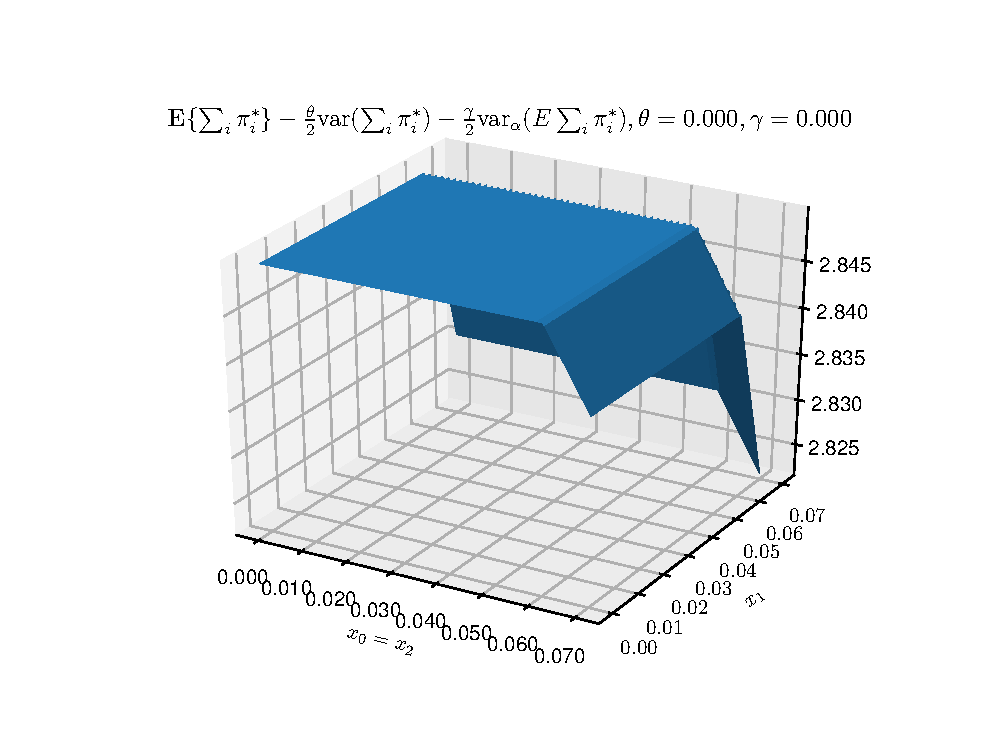
\includegraphics[width=0.7\textwidth]{Figures/AToy/Atoy-FCP000000} 
%   \caption{Optimal Expected utility}
%   \label{figOpExUt}
\end{figure}
\begin{figure}[htbp] %  figure placement: here, top, bottom, or page
   \centering
   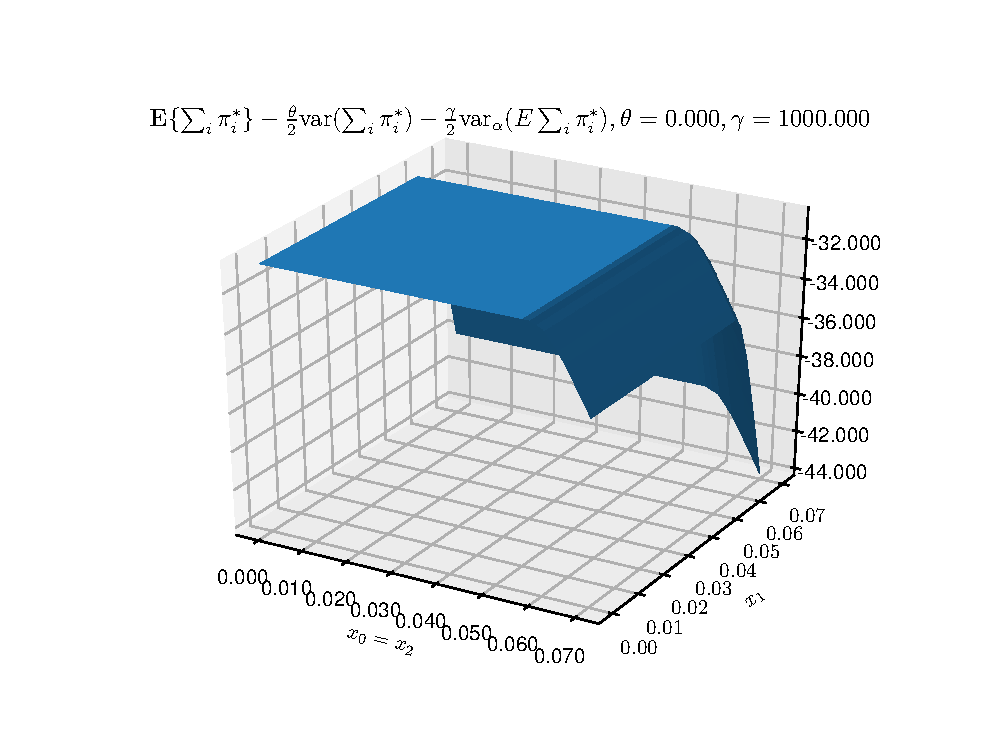
\includegraphics[width=0.7\textwidth]{Figures/AToy/Atoy-FCP000100000} 
%   \caption{Optimal Expected utility}
%   \label{figOpExUt}
\end{figure}

\begin{figure}[htbp] %  figure placement: here, top, bottom, or page
   \centering
   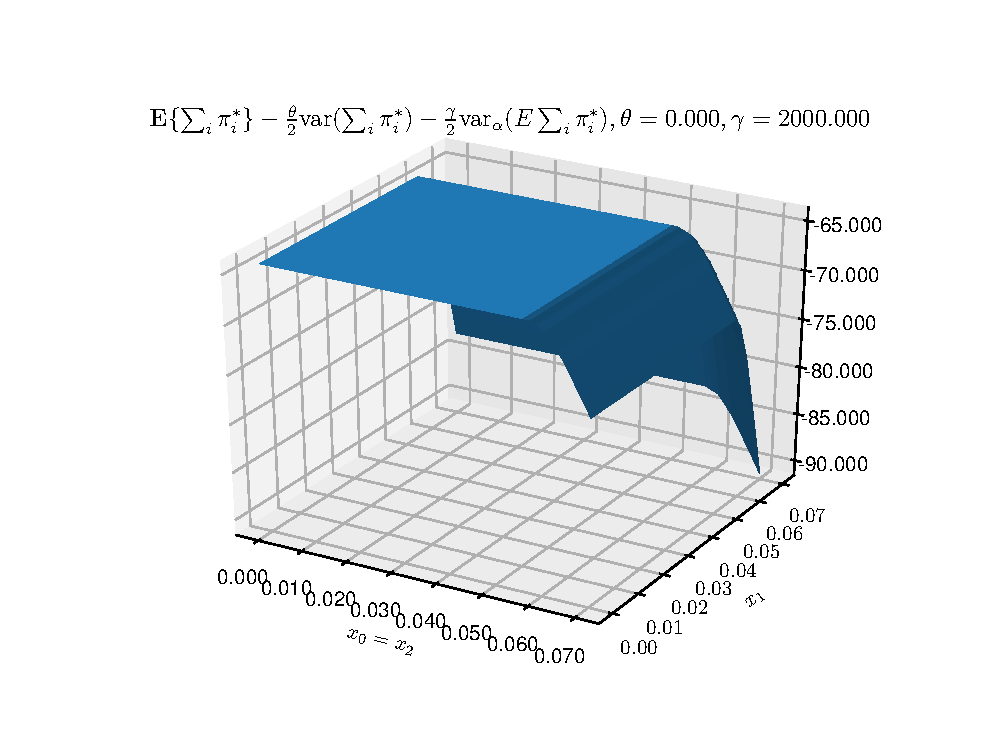
\includegraphics[width=0.7\textwidth]{Figures/AToy/Atoy-FCP000200000} 
%   \caption{Optimal Expected utility}
%   \label{figOpExUt}
\end{figure}

\begin{figure}[htbp] %  figure placement: here, top, bottom, or page
   \centering
   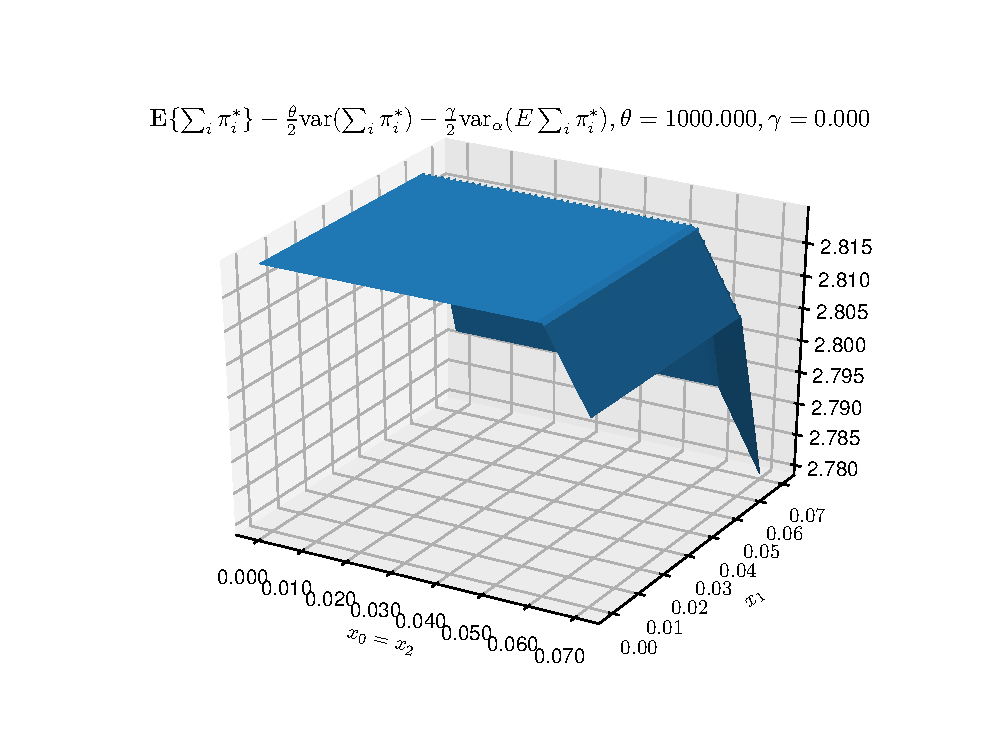
\includegraphics[width=0.7\textwidth]{Figures/AToy/Atoy-FCP100000000} 
%   \caption{Optimal Expected utility}
%   \label{figOpExUt}
\end{figure}

\begin{figure}[htbp] %  figure placement: here, top, bottom, or page
   \centering
   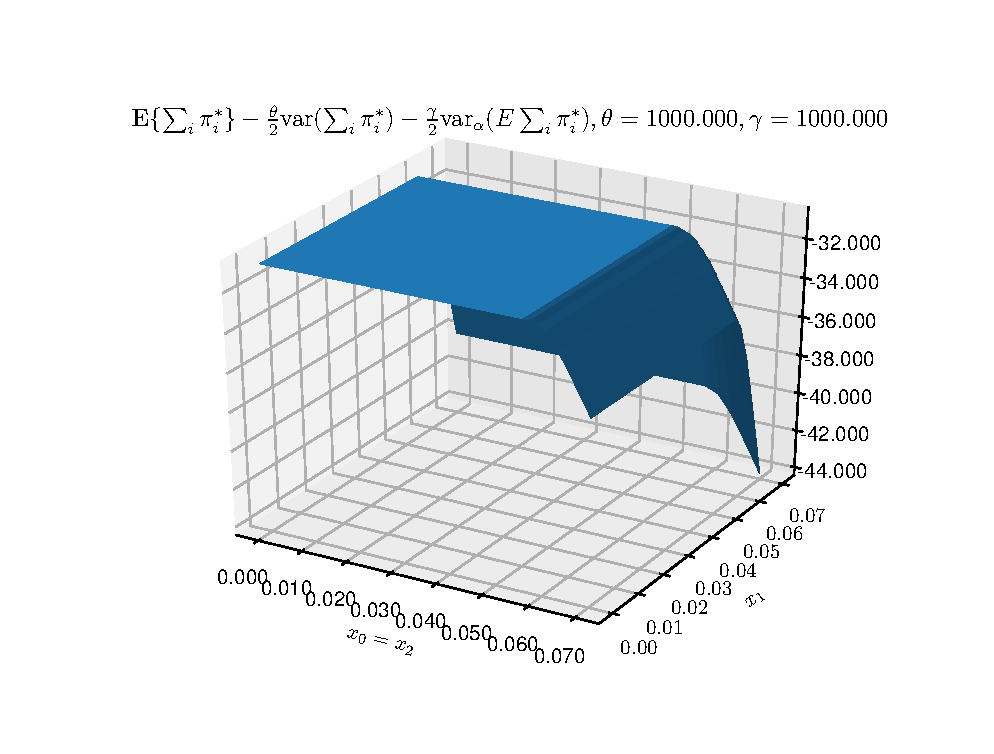
\includegraphics[width=0.7\textwidth]{Figures/AToy/Atoy-FCP100000100000} 
%   \caption{Optimal Expected utility}
%   \label{figOpExUt}
\end{figure}

\begin{figure}[htbp] %  figure placement: here, top, bottom, or page
   \centering
   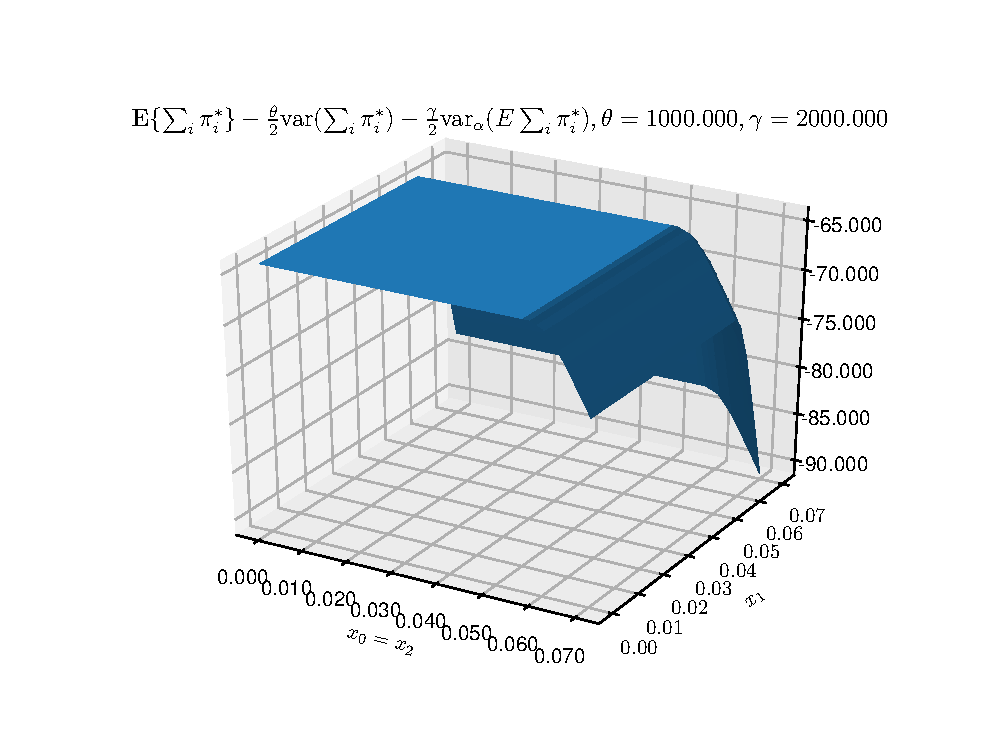
\includegraphics[width=0.7\textwidth]{Figures/AToy/Atoy-FCP100000200000} 
%   \caption{Optimal Expected utility}
%   \label{figOpExUt}
\end{figure}

\begin{figure}[htbp] %  figure placement: here, top, bottom, or page
   \centering
   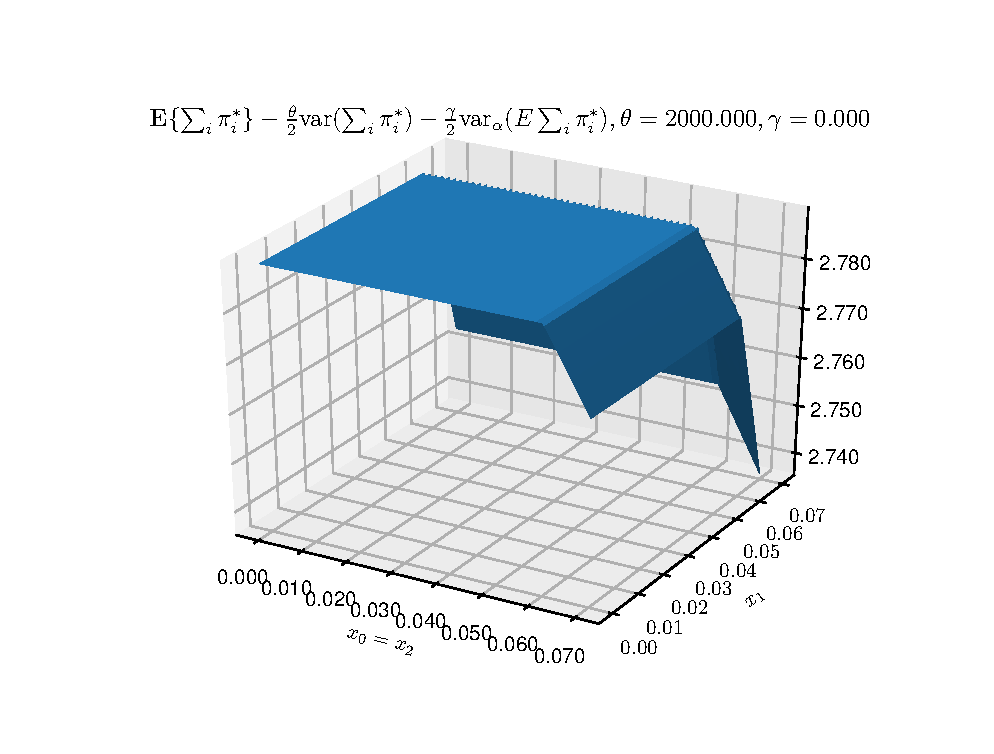
\includegraphics[width=0.7\textwidth]{Figures/AToy/Atoy-FCP200000000} 
%   \caption{Optimal Expected utility}
%   \label{figOpExUt}
\end{figure}


\begin{figure}[htbp] %  figure placement: here, top, bottom, or page
   \centering
   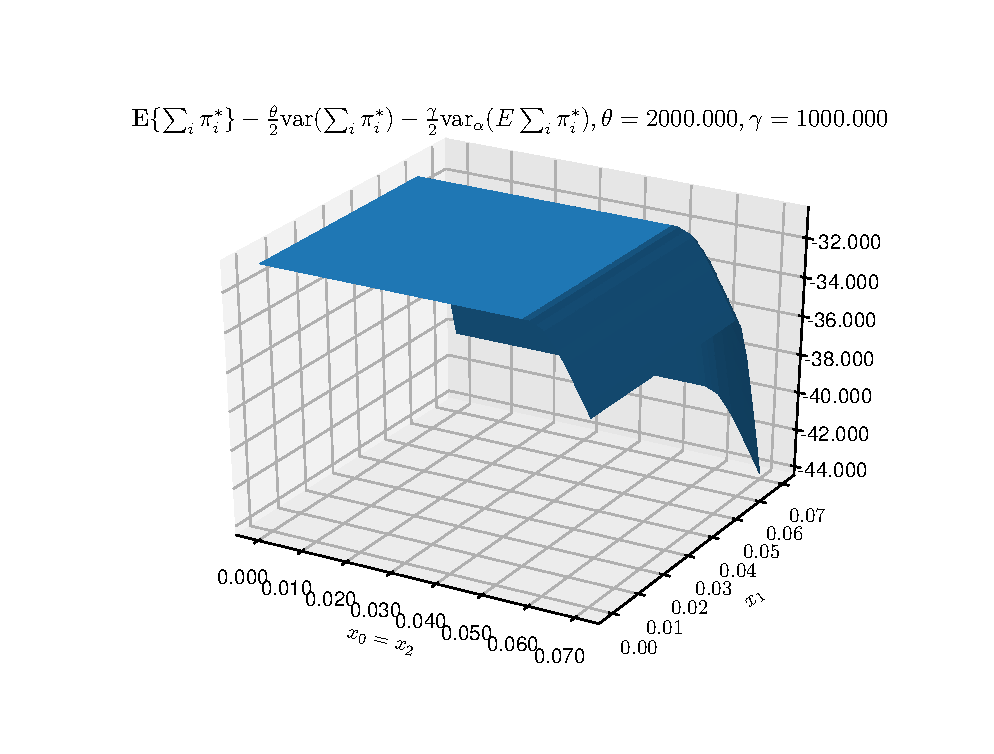
\includegraphics[width=0.7\textwidth]{Figures/AToy/Atoy-FCP200000100000} 
%   \caption{Optimal Expected utility}
%   \label{figOpExUt}
\end{figure}



\begin{figure}[htbp] %  figure placement: here, top, bottom, or page
   \centering
   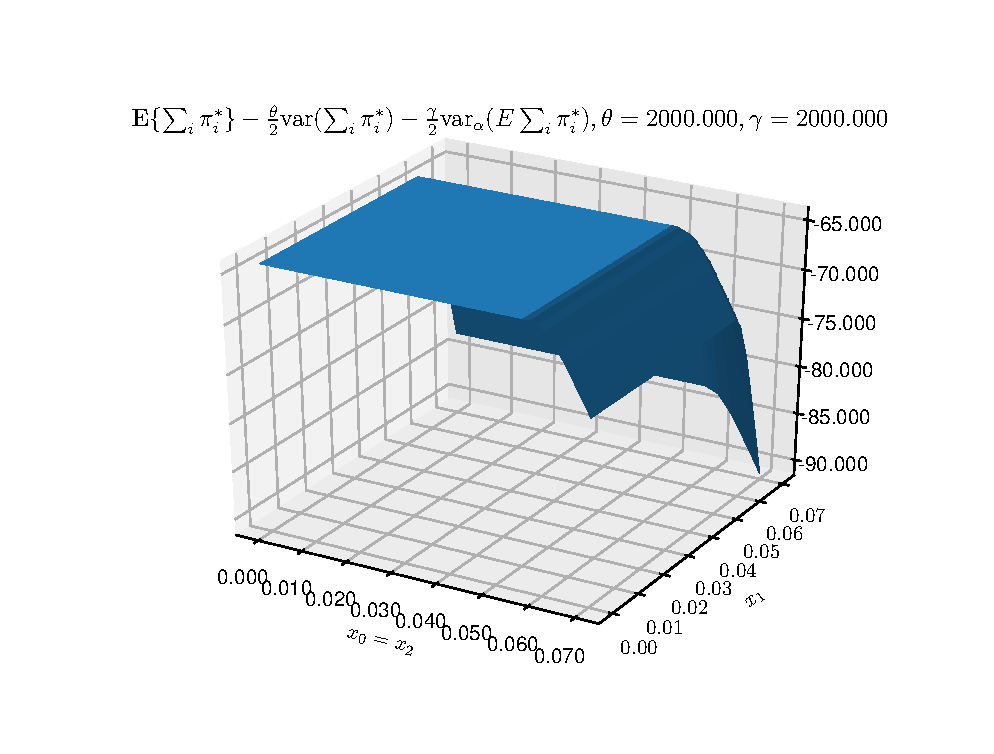
\includegraphics[width=0.7\textwidth]{Figures/AToy/Atoy-FCP200000200000} 
%   \caption{Optimal Expected utility}
%   \label{figOpExUt}
\end{figure}

\bibliographystyle{plain}
\bibliography{refer}


\end{document}
